\section{Appendix}
\label{sec:appendix}
\begin{figure*}
  \centering
  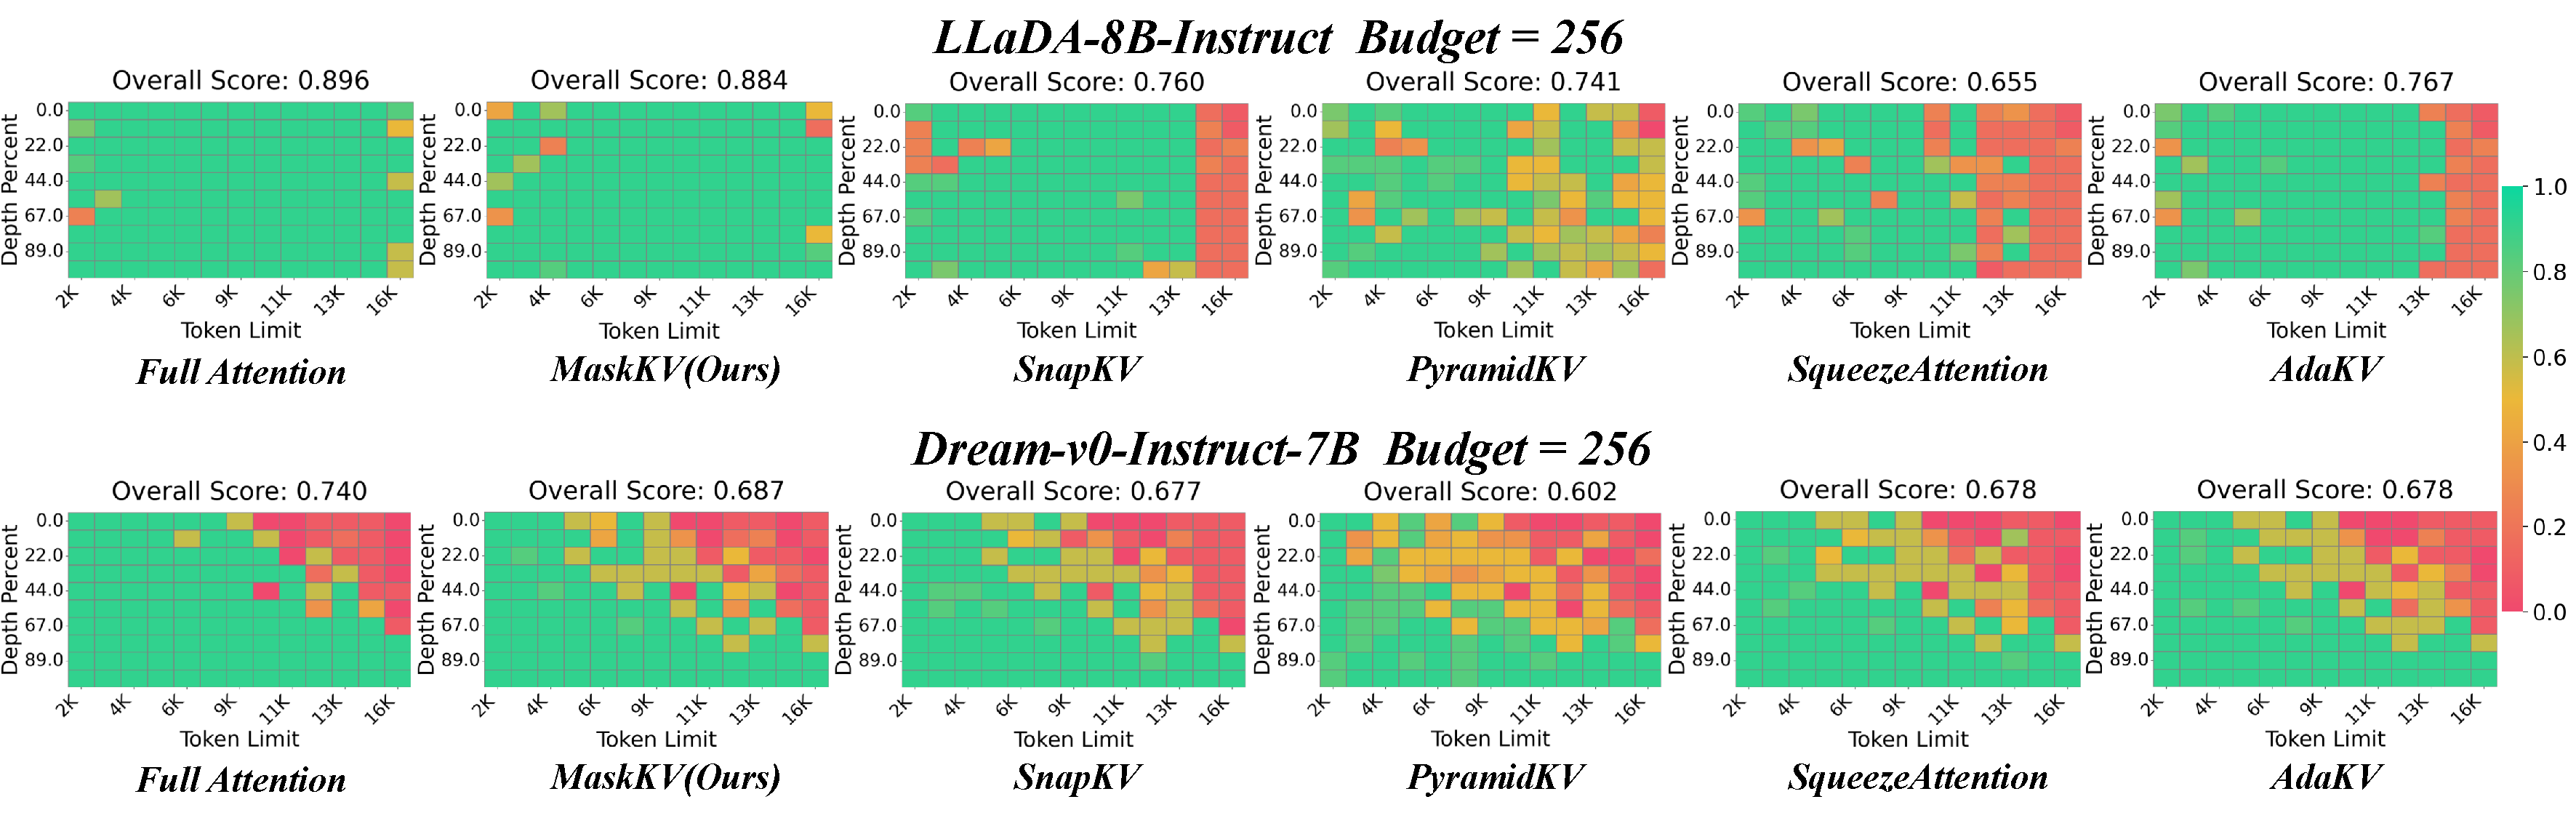
\includegraphics[width=1.0\linewidth]{figure/NIAH_a.pdf}
  \caption{Performance comparison of different KV Cache compression techniques on LLaDA-8B and Dream-7B models in the ``Needle-in-a-Haystack'' test (Budget B=256). The heatmaps show retrieval accuracy at different context lengths (x-axis) and depths (y-axis), where greener colors indicate better performance.}
  \label{fig:niah_all}
\end{figure*}

\begin{table*}[t!]
    \centering
    \small
    \caption{Detailed LongBench Results for LLaDA-8B-Instruct. Best result in each column within a budget section is in \textbf{bold}.}
    \label{tab:llada_full_longbench_results_final_reordered}
    
    \setlength{\tabcolsep}{3pt} 
    \renewcommand{\arraystretch}{1.1}
    
    \resizebox{\textwidth}{!}{%
    \begin{tabular}{@{}l*{15}{c}@{}}
        \toprule
        \textbf{Method} & \multicolumn{2}{c}{Single-Doc. QA} & \multicolumn{3}{c}{Multi-Doc. QA} & \multicolumn{3}{c}{Summarization} & \multicolumn{3}{c}{Few-shot Learning} & \multicolumn{1}{c}{Synthetic} & \multicolumn{2}{c}{Code} & \makecell{Ave. \\ Score} \\
        
        \cmidrule(lr){2-3} \cmidrule(lr){4-6} \cmidrule(lr){7-9} \cmidrule(lr){10-12} \cmidrule(lr){13-13} \cmidrule(lr){14-15}

        & \rotatebox[origin=c]{-45}{Qasper} & \rotatebox[origin=c]{-45}{MF-en} & \rotatebox[origin=c]{-45}{HotpotQA} 
        & \rotatebox[origin=c]{-45}{2WikiMQA} & \rotatebox[origin=c]{-45}{Musique} 
        & \rotatebox[origin=c]{-45}{GovReport} & \rotatebox[origin=c]{-45}{QMSum} & \rotatebox[origin=c]{-45}{MultiNews}
        & \rotatebox[origin=c]{-45}{TREC} & \rotatebox[origin=c]{-45}{TriviaQA} & \rotatebox[origin=c]{-45}{SAMSum}
        & \rotatebox[origin=c]{-45}{PRe}
        & \rotatebox[origin=c]{-45}{Lcc} & \rotatebox[origin=c]{-45}{RB-P}
        & \\
        
        \midrule
        \multicolumn{16}{c}{\large \textbf{LLaDA-8B-Instruct}} \\
        \midrule
        \multicolumn{16}{c}{\small Full KV Cache} \\
        \midrule
        dLLM w/o Cache & 16.96 & 31.31 & 14.68 & 17.60 & 11.48 & 29.24 & 21.93 & 27.58 & 65.20 & 47.98 & 40.51 & 98.17 & 65.69 & 59.57 & 39.14 \\
        dLLM w/ Cache & 15.26 & 29.62 & 13.87 & 17.17 & 10.44 & 29.75 & 22.06 & 26.68 & 66.00 & 44.94 & 41.86 & 97.44 & 66.07 & 59.34 & 38.61 \\
        \midrule
        \multicolumn{16}{c}{\small B=16} \\
        \midrule
        SnapKV & 10.66 & 12.28 & 12.96 & 13.18 & 4.91 & 7.59 & 9.85 & 11.80 & 21.25 & 49.98 & 14.37 & 31.50 & 30.75 & 24.17 & 18.23 \\
        PyramidKV & 7.94 & 8.34 & 10.95 & 8.77 & 4.80 & 7.61 & 9.02 & 10.98 & 14.75 & 46.29 & 12.71 & 24.00 & 30.48 & 23.94 & 15.76 \\
        SqueezeAttention & 8.27 & 10.49 & 14.28 & 14.19 & 5.47 & 7.27 & 7.92 & 11.98 & 31.25 & 42.39 & 13.83 & 30.25 & 29.49 & 22.73 & 17.84 \\
        AdaKV & 9.48 & 11.97 & 12.13 & \textbf{15.16} & 5.62 & 7.55 & \textbf{11.34} & 11.90 & 25.00 & 49.16 & 14.24 & 31.58 & 28.63 & 22.81 & 18.33 \\
        \rowcolor{lightgreen} \textbf{MaskKV (Ours)} & \textbf{16.11} & \textbf{19.81} & \textbf{18.24} & 14.16 & \textbf{11.40} & \textbf{7.86} & 8.31 & \textbf{13.69} & \textbf{28.50} & \textbf{52.32} & \textbf{23.29} & \textbf{87.00} & \textbf{50.09} & \textbf{37.32} & \textbf{27.72} \\
        \midrule
        \multicolumn{16}{c}{\small B=32} \\
        \midrule
        SnapKV & 9.10 & 17.49 & \textbf{17.38} & 16.45 & 8.06 & \textbf{9.92} & 12.21 & 13.95 & 39.25 & 54.32 & 16.41 & 55.00 & 39.90 & 29.08 & 24.18 \\
        PyramidKV & 9.90 & 12.12 & 14.46 & 14.62 & 8.18 & 9.10 & 8.83 & 12.36 & 26.42 & 53.26 & 14.51 & 28.00 & 39.18 & 27.66 & 19.90 \\
        SqueezeAttention & 11.49 & 14.72 & 16.66 & 15.42 & 8.15 & 9.28 & 10.49 & 14.86 & 43.50 & 53.67 & 15.73 & 52.00 & 33.60 & 25.56 & 23.22 \\
        AdaKV & 11.15 & 16.21 & 16.69 & \textbf{16.98} & 7.48 & 9.10 & 10.44 & 14.23 & 39.17 & \textbf{55.69} & 19.00 & 59.50 & 37.21 & 26.40 & 24.23 \\
        \rowcolor{lightgreen} \textbf{MaskKV (Ours)} & \textbf{14.61} & \textbf{24.45} & 17.05 & 15.68 & \textbf{12.50} & 9.54 & \textbf{14.33} & \textbf{16.43} & \textbf{40.42} & 54.64 & \textbf{29.28} & \textbf{90.33} & \textbf{56.08} & \textbf{42.21} & \textbf{31.25} \\
        \midrule
        \multicolumn{16}{c}{\small B=64} \\
        \midrule
        SnapKV & 13.77 & 23.25 & 17.12 & \textbf{18.74} & 8.74 & 10.55 & 10.78 & 16.67 & 46.83 & 56.95 & 19.79 & 73.00 & 48.94 & 33.75 & 28.49 \\
        PyramidKV & 12.23 & 21.13 & 15.95 & 16.90 & 8.64 & 9.42 & 9.24 & 15.02 & 37.25 & 56.70 & 18.70 & 51.00 & 49.73 & 34.53 & 25.46 \\
        SqueezeAttention & 11.30 & 17.71 & 17.68 & 18.32 & 9.49 & 11.20 & 11.60 & 17.61 & 44.79 & 54.58 & 16.51 & 66.00 & 38.64 & 29.51 & 26.07 \\
        AdaKV & 13.21 & 22.39 & \textbf{19.60} & 17.56 & 8.25 & 10.50 & 9.25 & 17.25 & 47.17 & \textbf{57.65} & 20.15 & 71.50 & 47.88 & 30.44 & 28.06 \\
        \rowcolor{lightgreen} \textbf{MaskKV (Ours)} & \textbf{18.48} & \textbf{27.42} & 19.00 & 16.04 & \textbf{10.12} & \textbf{10.93} & \textbf{17.25} & \textbf{18.88} & \textbf{55.08} & 50.98 & \textbf{33.47} & \textbf{95.08} & \textbf{59.71} & \textbf{46.80} & \textbf{34.23} \\
        \midrule
        \multicolumn{16}{c}{\small B=128} \\
        \midrule
        SnapKV & 17.42 & 26.65 & 15.88 & 17.44 & 7.99 & 11.50 & 11.69 & 18.89 & 50.83 & 55.60 & 20.72 & 80.00 & 54.90 & 39.33 & 30.63 \\
        PyramidKV & 15.71 & 25.20 & 16.22 & 16.20 & 8.47 & 10.09 & 11.06 & 17.22 & 39.92 & 55.03 & 23.49 & 83.25 & 54.00 & 40.50 & 29.74 \\
        SqueezeAttention & 14.46 & 17.64 & \textbf{18.12} & \textbf{17.97} & 8.00 & 13.46 & 10.69 & 19.46 & 52.67 & 54.71 & 17.04 & 71.00 & 48.30 & 32.51 & 28.29 \\
        AdaKV & 19.42 & 24.68 & 17.06 & 17.57 & 8.82 & 11.85 & 9.51 & 18.49 & 49.92 & \textbf{57.90} & 21.03 & 78.00 & 54.64 & 36.27 & 30.37 \\
        \rowcolor{lightgreen} \textbf{MaskKV (Ours)} & \textbf{20.21} & \textbf{29.84} & 15.78 & 16.65 & \textbf{11.83} & \textbf{13.60} & \textbf{17.67} & \textbf{20.78} & \textbf{57.00} & 46.06 & \textbf{37.28} & \textbf{98.17} & \textbf{61.61} & \textbf{51.86} & \textbf{35.60} \\
        \midrule
        \multicolumn{16}{c}{\small B=256} \\
        \midrule
        SnapKV & 19.74 & 27.33 & 16.62 & \textbf{18.41} & \textbf{10.35} & 12.12 & 12.03 & 21.00 & 47.63 & 53.29 & 26.53 & 92.92 & 58.93 & 42.95 & 32.85 \\
        PyramidKV & 18.50 & 29.07 & 14.61 & 16.05 & 8.92 & 12.65 & 12.15 & 19.22 & 43.17 & 52.17 & 29.09 & 91.33 & 56.54 & 43.89 & 31.95 \\
        SqueezeAttention & 19.35 & 23.79 & 16.69 & 16.35 & 8.78 & 13.75 & 11.24 & 21.43 & 51.50 & \textbf{54.12} & 21.48 & 77.25 & 57.08 & 36.91 & 30.69 \\
        AdaKV & 19.52 & 27.73 & 16.14 & 17.36 & 9.89 & 12.12 & 11.41 & 20.13 & 51.25 & 53.88 & 25.87 & 96.25 & 58.30 & 40.78 & 32.90 \\
        \rowcolor{lightgreen} \textbf{MaskKV (Ours)} & \textbf{22.71} & \textbf{29.72} & \textbf{14.81} & 16.77 & 9.19 & \textbf{16.69} & \textbf{20.18} & \textbf{23.14} & \textbf{62.25} & 41.65 & \textbf{40.48} & \textbf{98.92} & \textbf{61.23} & \textbf{52.20} & \textbf{36.42} \\
        \midrule
        \multicolumn{16}{c}{\small B=512} \\
        \midrule
        SnapKV & 19.98 & 30.03 & 12.89 & 16.93 & \textbf{10.32} & 15.66 & 13.21 & 23.36 & 49.17 & 52.09 & 32.71 & 98.00 & 61.24 & 45.37 & 34.35 \\
        PyramidKV & 19.53 & 29.23 & 14.06 & 14.75 & 9.31 & 15.45 & 13.93 & 21.81 & 52.67 & 46.03 & 35.28 & \textbf{100.00} & 59.28 & 45.58 & 34.07 \\
        SqueezeAttention & \textbf{20.71} & 26.45 & \textbf{16.44} & \textbf{17.70} & 8.04 & 14.69 & 12.23 & 23.54 & 55.92 & 50.13 & 29.29 & 96.75 & 61.08 & 45.01 & 34.14 \\
        AdaKV & 19.65 & \textbf{31.77} & 13.47 & 16.10 & 9.97 & 14.53 & 13.41 & 22.34 & 50.25 & 52.06 & 33.31 & 96.00 & 60.95 & 44.27 & 34.15 \\
        \rowcolor{lightgreen} \textbf{MaskKV (Ours)} & 17.85 & 28.92 & 13.85 & 17.10 & 8.93 & \textbf{18.58} & \textbf{20.29} & \textbf{25.05} & \textbf{64.25} & \textbf{41.62} & \textbf{41.04} & 99.33 & \textbf{62.46} & \textbf{53.78} & \textbf{36.65} \\

        \bottomrule
    \end{tabular}
    } 
\end{table*}
\begin{table*}[t!]
    \centering
    \small
    \caption{Detailed LongBench Results for Dream-v0-Instruct-7B. Best result in each column within a budget section is in \textbf{bold}.}
    \label{tab:dream_full_longbench_results_final_verified}
    
    \setlength{\tabcolsep}{3pt} 
    \renewcommand{\arraystretch}{1.1}
    
    \resizebox{\textwidth}{!}{%
    \begin{tabular}{@{}l*{15}{c}@{}}
        \toprule
        \textbf{Method} & \multicolumn{2}{c}{Single-Doc. QA} & \multicolumn{3}{c}{Multi-Doc. QA} & \multicolumn{3}{c}{Summarization} & \multicolumn{3}{c}{Few-shot Learning} & \multicolumn{1}{c}{Synthetic} & \multicolumn{2}{c}{Code} & \makecell{Ave. \\ Score} \\
        
        \cmidrule(lr){2-3} \cmidrule(lr){4-6} \cmidrule(lr){7-9} \cmidrule(lr){10-12} \cmidrule(lr){13-13} \cmidrule(lr){14-15}

        & \rotatebox[origin=c]{-45}{Qasper} & \rotatebox[origin=c]{-45}{MF-en} & \rotatebox[origin=c]{-45}{HotpotQA} 
        & \rotatebox[origin=c]{-45}{2WikiMQA} & \rotatebox[origin=c]{-45}{Musique} 
        & \rotatebox[origin=c]{-45}{GovReport} & \rotatebox[origin=c]{-45}{QMSum} & \rotatebox[origin=c]{-45}{MultiNews}
        & \rotatebox[origin=c]{-45}{TREC} & \rotatebox[origin=c]{-45}{TriviaQA} & \rotatebox[origin=c]{-45}{SAMSum}
        & \rotatebox[origin=c]{-45}{PRe}
        & \rotatebox[origin=c]{-45}{Lcc} & \rotatebox[origin=c]{-45}{RB-P}
        & \\
        
        \midrule
        \multicolumn{16}{c}{\large \textbf{Dream-v0-Instruct-7B}} \\
        \midrule
        \multicolumn{16}{c}{\small Full KV Cache} \\
        \midrule
        dLLM w/o Cache & 28.17 & 36.23 & 27.65 & 32.43 & 11.83 & 5.04 & 14.29 & 5.95 & 73.00 & 89.25 & 37.84 & 16.92 & 38.91 & 45.08 & 33.04 \\
        dLLM w/ Cache & 26.55 & 39.86 & 27.66 & 32.09 & 11.12 & 4.40 & 13.89 & 5.51 & 73.50 & 89.59 & 36.07 & 12.05 & 39.88 & 45.57 & 32.70 \\
        \midrule
        \multicolumn{16}{c}{\small B=16} \\
        \midrule
        SnapKV & \textbf{15.36} & 18.35 & 11.98 & 9.92 & 5.27 & 2.56 & 10.88 & 1.91 & 26.50 & 27.14 & 19.42 & 3.56 & 17.28 & 16.08 & 13.30 \\
        PyramidKV & 10.81 & 12.81 & 12.82 & 6.40 & 3.95 & \textbf{2.57} & 10.55 & 1.89 & 26.50 & 8.05 & 17.98 & 0.00 & 15.54 & 15.19 & 10.36 \\
        SqueezeAttention & 12.39 & 16.36 & 11.21 & 6.25 & 3.95 & 2.54 & 10.60 & 1.87 & 26.50 & 10.26 & 18.35 & 3.06 & 13.66 & 13.60 & 10.76 \\
        AdaKV & 15.31 & 15.14 & 12.18 & 8.50 & 6.44 & 2.54 & 10.79 & 1.82 & 26.50 & 21.56 & 20.08 & 5.11 & 16.91 & 17.10 & 12.86 \\
        \rowcolor{lightgreen} \textbf{MaskKV (Ours)} & 12.63 & \textbf{25.72} & \textbf{23.87} & \textbf{20.99} & \textbf{8.53} & 2.56 & \textbf{11.15} & \textbf{2.02} & \textbf{27.50} & \textbf{79.07} & \textbf{24.30} & \textbf{13.50} & \textbf{20.57} & \textbf{21.40} & \textbf{20.99} \\
        \midrule
        \multicolumn{16}{c}{\small B=32} \\
        \midrule
        SnapKV & 17.75 & 26.82 & 22.39 & \textbf{27.91} & 7.53 & \textbf{2.65} & \textbf{12.58} & 1.95 & 28.25 & 66.14 & 23.67 & 17.50 & 22.75 & 23.87 & 21.55 \\
        PyramidKV & 14.55 & 24.51 & 22.41 & 15.27 & 6.90 & 2.62 & 11.89 & 2.15 & 28.00 & 57.55 & 24.17 & 11.50 & 22.02 & 22.22 & 18.98 \\
        SqueezeAttention & 17.62 & 30.44 & 20.07 & 26.15 & 7.42 & 2.62 & 11.83 & 2.19 & 26.25 & 72.17 & 24.52 & 17.00 & 20.91 & 23.41 & 22.00 \\
        AdaKV & 17.09 & 25.42 & 23.64 & 24.77 & 7.55 & 2.58 & 12.46 & 1.89 & 27.75 & 69.77 & 25.21 & 18.83 & 21.67 & 24.98 & 21.69 \\
        \rowcolor{lightgreen} \textbf{MaskKV (Ours)} & \textbf{18.53} & \textbf{33.76} & \textbf{32.92} & 24.53 & \textbf{11.02} & 2.59 & 11.98 & \textbf{2.25} & \textbf{33.25} & \textbf{86.47} & \textbf{27.55} & \textbf{20.00} & \textbf{24.89} & \textbf{27.40} & \textbf{25.51} \\
        \midrule
        \multicolumn{16}{c}{\small B=64} \\
        \midrule
        SnapKV & 19.61 & 34.91 & 31.26 & 28.17 & 10.51 & 2.65 & 12.81 & 2.28 & 34.25 & 81.68 & 27.56 & \textbf{24.00} & 28.07 & 30.02 & 26.27 \\
        PyramidKV & 16.33 & 29.06 & 24.28 & 18.74 & 8.61 & \textbf{2.70} & 12.73 & 2.60 & 33.67 & 72.43 & 26.87 & 23.00 & 25.47 & 26.78 & 23.09 \\
        SqueezeAttention & 17.62 & 30.44 & 23.42 & 26.15 & 8.75 & 2.62 & 12.58 & 2.19 & 26.25 & 72.17 & 24.52 & 17.00 & 20.91 & 23.41 & 22.00 \\
        AdaKV & 20.98 & 36.31 & 33.10 & 29.06 & 9.55 & 2.59 & \textbf{13.12} & 2.29 & 35.25 & 85.24 & 28.50 & \textbf{24.00} & 28.09 & \textbf{32.76} & 27.20 \\
        \rowcolor{lightgreen} \textbf{MaskKV (Ours)} & \textbf{22.73} & \textbf{37.98} & \textbf{36.47} & \textbf{31.03} & \textbf{12.26} & 2.68 & 12.39 & \textbf{2.77} & \textbf{45.00} & \textbf{87.36} & \textbf{29.98} & 22.50 & \textbf{29.11} & 31.61 & \textbf{28.85} \\
        \midrule
        \multicolumn{16}{c}{\small B=128} \\
        \midrule
        SnapKV & \textbf{22.36} & 39.02 & 30.28 & 32.27 & 11.51 & 2.72 & \textbf{13.20} & 2.72 & 38.00 & 87.17 & 28.69 & \textbf{26.05} & \textbf{32.55} & 36.51 & 28.79 \\
        PyramidKV & 17.31 & 36.59 & 25.21 & 24.38 & 10.99 & 2.77 & 12.75 & 2.90 & 39.75 & 84.83 & 29.71 & 24.00 & 30.26 & 30.33 & 26.56 \\
        SqueezeAttention & 19.36 & 36.19 & 28.35 & 29.79 & 10.25 & 2.81 & 13.11 & 2.64 & 33.00 & 85.99 & 29.25 & 25.00 & 27.11 & 31.92 & 26.77 \\
        AdaKV & 21.97 & \textbf{39.68} & 33.24 & 31.57 & 11.38 & 2.69 & 13.15 & 2.80 & 38.75 & 88.51 & 30.43 & 24.25 & 31.46 & \textbf{37.28} & 29.08 \\
        \rowcolor{lightgreen} \textbf{MaskKV (Ours)} & 21.49 & 39.23 & \textbf{38.25} & \textbf{33.99} & \textbf{14.76} & \textbf{2.86} & 12.48 & \textbf{3.19} & \textbf{53.50} & \textbf{88.69} & \textbf{30.97} & 21.92 & 30.71 & 34.79 & \textbf{30.49} \\
        \midrule
        \multicolumn{16}{c}{\small B=256} \\
        \midrule
        SnapKV & 23.01 & 40.81 & 35.52 & 33.92 & 12.08 & 2.89 & 13.06 & 3.33 & 44.75 & 89.57 & 32.16 & 21.65 & \textbf{35.49} & 37.61 & 30.42 \\
        PyramidKV & 21.50 & 36.74 & 28.35 & 29.08 & 9.17 & 2.79 & 13.06 & 3.55 & 46.17 & 88.44 & 31.74 & 22.25 & 32.78 & 33.09 & 28.55 \\
        SqueezeAttention & 21.82 & 41.20 & 35.80 & 33.23 & 11.36 & 2.83 & 13.11 & 2.56 & 37.00 & \textbf{89.63} & 30.79 & \textbf{25.00} & 30.29 & 34.69 & 29.24 \\
        AdaKV & 24.00 & \textbf{43.32} & 35.86 & 33.75 & 11.97 & 2.90 & \textbf{13.14} & 3.41 & 48.50 & 87.70 & 32.66 & 19.96 & 35.40 & \textbf{39.41} & 30.86 \\
        \rowcolor{lightgreen} \textbf{MaskKV (Ours)} & \textbf{24.13} & 39.43 & \textbf{36.47} & \textbf{31.93} & \textbf{12.66} & \textbf{2.93} & 12.90 & \textbf{3.74} & \textbf{58.00} & 88.52 & \textbf{32.93} & 20.58 & 32.22 & 35.94 & \textbf{30.88} \\
        \midrule
        \multicolumn{16}{c}{\small B=512} \\
        \midrule
        SnapKV & 24.27 & 40.23 & 35.32 & 34.87 & 11.65 & 2.91 & 13.32 & 4.15 & 51.00 & \textbf{89.66} & 33.09 & 16.29 & 37.22 & 40.47 & 31.03 \\
        PyramidKV & 21.50 & 36.74 & 28.35 & 29.08 & 9.17 & 2.79 & 13.06 & 3.55 & 46.17 & 88.44 & 31.74 & \textbf{22.25} & 32.78 & 33.09 & 28.55 \\
        SqueezeAttention & 22.17 & 40.15 & 35.98 & \textbf{35.63} & 11.32 & 2.89 & 13.19 & 3.91 & 45.00 & 86.95 & 32.37 & 17.08 & 33.04 & 38.75 & 29.89 \\
        AdaKV & 23.86 & \textbf{40.62} & \textbf{37.45} & 34.66 & 12.58 & 3.05 & \textbf{13.61} & 3.81 & 57.75 & 89.15 & 33.50 & 17.42 & \textbf{37.23} & \textbf{42.35} & \textbf{31.93} \\
        \rowcolor{lightgreen} \textbf{MaskKV (Ours)} & \textbf{25.90} & 39.71 & 33.27 & 34.01 & \textbf{13.68} & \textbf{3.10} & 12.92 & \textbf{4.26} & \textbf{60.75} & 87.49 & \textbf{33.78} & 16.81 & 34.19 & 38.83 & 31.34 \\

        \bottomrule
    \end{tabular}
    } 
\end{table*}

\begin{table}[t!]
\caption{Comparison of \textbf{dLLM-Cache} with its simplified variants.}
\label{tab:ablation_memory}
\centering
\begin{tabular}{l c}
\toprule
\textbf{Method} & \textbf{Memory (GB)} \\
\midrule
\textbf{dLLM-Cache}                            & 68.13 \\
\midrule
\quad + Mask-Only Projection                 & 53.74 \\
\quad + Prompt state exclusion             & 38.12 \\
\quad + \mymethod (online)                            & 38.12 \\
\quad + \mymethod (offline)                            & \textbf{23.42} \\
\bottomrule
\end{tabular}
\end{table}

\subsection{Details of \emph{MaskKV}}
\label{sec:maskkv_details}
\paragraph{Prompt-state Exclusion.}
In dLLM-Cache, features from both the prompt and response tokens (including keys, values, attention outputs, and MLP activations) are cached at each denoising step.
However, we observe that only the key–value representations of prompt tokens contribute to the attention computation of mask tokens, while the prompt-side attention and MLP outputs have no downstream influence.
We therefore exclude these redundant prompt features from caching and retain only their key–value pairs, which substantially reduces memory usage without affecting generation quality.

\paragraph{Mask-only Projection.}
In the official LLaDA implementation, after the final layer computation, the model projects all tokens (including both prompt and mask positions) into the vocabulary space to produce logits.
This operation yields a large but unnecessary tensor, as the logits of prompt tokens are never used during decoding.
We thus restrict the vocabulary projection to masked positions only and skip the prompt ones.
This \emph{mask-only projection} optimization removes redundant matrix multiplications and further reduces GPU memory consumption.

\subsection{Implementation Details}
\label{implement details}
\paragraph{Evaluation Metrics.}
We evaluate both the efficiency and quality of our method using quantitative metrics. 
Generation quality is assessed with the official task-specific metrics (see Table~\ref{tab:longbench_datasets_simplified} for details) of LongBench, which measure model accuracy under cache eviction.  
Computation efficiency is reported in Tokens Per Second (TPS), reflecting the average number of tokens decoded per second.  
For memory efficiency, we track both the peak GPU memory during inference and the size of the KV cache.  
Under bf16 precision, the KV cache memory footprint is given by  
\begin{equation}
\text{Mem}_{\text{KV}} = 2 \cdot L \cdot H \cdot d_{\text{head}} \cdot s_{\text{bf16}},
\end{equation}
where $L$ is the sequence length, $H$ the number of attention heads, $d_{\text{head}}$ the dimension per head, and $s_{\text{bf16}}=2$ bytes denotes the storage size of a \texttt{bf16} element.  
The factor $2$ represents the storage requirements for both key and value states.

\paragraph{Baseline.}
We compare one token-selection scheme and three architectural budget-allocation policies under an identical cache budget, enabling a fair, apples-to-apples assessment of their effectiveness. \\
For the token selection strategy, we evaluate one strong KV-cache compression method as a baseline for autoregressive models.
\begin{itemize}
  \item \textbf{SnapKV} uses a small ``observation window'' at the end of the prompt to predict which parts of the entire context are most important. It analyzes the attention scores from this window in ``voting'' mechanism to identify and select these key parts.
\end{itemize}
For architectural budget allocation, we evaluate competitive approaches that distribute the budget across the model's various structural components.
\begin{itemize}
  \item \textbf{PyramidKV} implements a static, non-uniform budget allocation where the cache capacity of each layer is a direct function of its depth. This function is engineered to be monotonically decreasing, granting the maximal budget to the lowest layers and progressively constricting it for higher layers that process more semantically aggregated representations.
  \item \textbf{SqueezeAttention} gauges layer importance by calculating the cosine similarity between the input and output of an attention block. Based on this score, it classifies layers into three tiers and assigns a minimal cache budget to the least important one.
  \item \textbf{Ada-KV} allocates its cache budget in a fine-grained, adaptive manner: it first assesses the relative importance of each key–value (KV) pair across all attention heads, then distributes the budget proportionally, granting a larger share of resources to KVs belonging to the most salient heads.
\end{itemize}


\paragraph{Parameters.}
Our experimental parameters are configured in accordance with prior research\citep{li2024snapkv, cai2024pyramidkv,wang2024squeezeattention, feng2024ada}. The specific settings are as follows:

\begin{itemize}
    \item \textbf{Default Selection Method}: Unless otherwise specified, we adopt \textbf{SnapKV} as the foundational selection method for all budget allocation strategies. For SnapKV~\citep{li2024snapkv} itself, the final window size is set to \textbf{32}, consistent with its application in the LongBench benchmark.
    \item \textbf{Pyramid-based Allocation}: We set the hyperparameter $\beta$, which directly controls the ``steepness''
    of the allocation pyramid, to \textbf{20}, adhering to the default value proposed in the original paper~\citep{cai2024pyramidkv}.
    \item \textbf{SqueezeAttention}: We cluster the layers into three distinct groups. A \textbf{40\%} budget is allocated to the least important group, a setting identified as optimal in its original study.
    \item \textbf{AdaKV}\citep{feng2024ada}: We reserve a \textbf{20\%} budget for uniform allocation. This measure is implemented to prevent the assignment of excessively small budgets to highly sparse attention heads.
\end{itemize}


\paragraph{Experiment settings.}
To ensure reproducibility, we outline our experimental settings. Unless otherwise specified, our default configuration sets the prompt refresh interval to 50, the response refresh interval to 5, the transfer ratio to 0.25, and the block length to 8. The step size is set equal to the generation length, which is specified for each task in Table~\ref{tab:longbench_datasets_simplified}.
For the results presented in Fig.~\ref{fig:across_size} and the ablation study in Tab.~\ref{tab:ablation}, the KV cache budget is set to 256. The experiment in Fig.~\ref{fig:hy}~ is conducted on the HotpotQA dataset with a budget of 32. For the NIAH baseline, we adopt the same configuration as that used in DuoAttention~\citep{xiao2024duoattention}.





\paragraph{Datasets.}

We conducted evaluations using LongBench~\citep{bai2023longbench}.
The LongBench benchmark \citep{bai2023longbench} evaluates large language models across a diverse set of long-context tasks. The benchmark is structured into six key domains:
\begin{itemize}
    \item \textbf{Single-Document QA:} Assesses a model's ability to extract answers from a single source document. This category utilizes datasets such as NarrativeQA~\citep{kovcisky2018narrativeqa}, Qasper~\citep{dasigi2021dataset}, and MultiFieldQA~\citep{bai2023longbench}, covering documents ranging from academic papers and legal files to encyclopedias.

    \item \textbf{Multi-Document QA:} Challenges models to synthesize information from multiple documents to formulate a coherent answer. It employs Wikipedia-based multi-hop QA datasets, including HotpotQA~\citep{yang2018hotpotqa}, 2WikiMultihopQA~\citep{ho2020constructing}, and MuSiQue~\citep{trivedi2022musique}.

    \item \textbf{Summarization:} Tests a model's capacity for comprehensive understanding and condensation of long texts. The datasets for this task are GovReport~\citep{huang2021efficient}, QMSum~\citep{zhong2021qmsum}, and the multi-document corpus MultiNews~\citep{fabbri2019multi}.

    \item \textbf{Few-shot Learning:} Measures a model's adaptability on a variety of tasks with limited examples. This includes classification with TREC~\citep{li2002learning}, conversational summarization with SAMSum~\citep{gliwa2019samsum}, and reading comprehension with TriviaQA~\citep{joshi2017triviaqa}.
    
    \item \textbf{Synthetic Tasks:} Purpose-built challenges designed to test specific abilities, such as counting unique passages (PassageCount~\citep{bai2023longbench}) or matching a summary to its source passage (PassageRetrieval-en~\citep{raffel2020exploring}).

    \item \textbf{Code Completion:} Evaluates a model's proficiency in generating code based on existing context. This is tested using the LCC~\citep{guo2023longcoder} dataset for single-file contexts and the RepoBench-P~\citep{liu2023repobench} dataset for tasks requiring information aggregation across multiple files.
\end{itemize}
\begin{table*}
    \centering
    \caption{Detailed information of the datasets in the LongBench benchmark.}
    \label{tab:longbench_datasets_simplified}
    \setlength{\tabcolsep}{5pt} 
    % 在这里增加了一个 'r' 列
    \begin{tabular}{lllrcrcr}
        \toprule
        \textbf{Label} & \textbf{Task} & \textbf{Eval Metric} & \textbf{Avg Len} & \textbf{Gen Len} & \textbf{Language} & \textbf{Sample Num} \\
        \midrule
        NrtvQA & NarrativeQA & F1 & 18,409 & 128 & EN & 200 \\
        Qasper & Qasper & F1 & 3,619 & 128 & EN & 200 \\
        MF-en & MultiFieldQA-en & F1 & 4,559 & 64 & EN & 150 \\
        HotpotQA & HotpotQA & F1 & 9,151 & 32 & EN & 200 \\
        2WikiMQA & 2WikiMultihopQA & F1 & 4,887 & 32 & EN & 200 \\
        Musique & MuSiQue & F1 & 11,214 & 32 & EN & 200 \\
        GovReport & GovReport & Rouge-L & 8,734 & 512 & EN & 200 \\
        QMSum & QMSum & Rouge-L & 10,614 & 512 & EN & 200 \\
        MultiNews & MultiNews & Rouge-L & 2,113 & 512 & EN & 200 \\
        TREC & TREC & Accuracy & 5,177 & 64 & EN & 200 \\
        TriviaQA & TriviaQA & F1 & 8,209 & 32 & EN & 200 \\
        SAMSum & SAMSum & Rouge-L & 6,258 & 128 & EN & 200 \\
        PCount & PassageCount & Accuracy & 11,141 & 32 & EN & 200 \\
        PRe & PassageRetrieval-en & Accuracy & 9,289 & 32 & EN & 200 \\
        Lcc & LCC & Edit Sim & 1,235 & 64 & Python/C\#/Java & 500 \\
        RB-P & RepoBench-P & Edit Sim & 4,206 & 64 & Python/Java & 500 \\
        \bottomrule
    \end{tabular}
\end{table*}



% -------------------------------

\subsection{A Formal Proof on the Primacy of Mask Attention}
\label{the primacy of mask attention}
\subsubsection{Preliminaries and Notation}

To ensure the rigor of the proof, we first define the symbols and notation used throughout this section.
\begin{itemize}
    \item \textbf{Input Sequence:} The input sequence $X \in \mathbb{R}^{n \times d}$ consists of embeddings for $n$ tokens, where $d$ is the embedding dimension. The sequence $X$ is partitioned into two parts:
    \begin{itemize}
        \item \textbf{Prompt:} $X_p \in \mathbb{R}^{n_p \times d}$, with its set of token indices denoted as $S_p$.
        \item \textbf{Mask:} $X_m \in \mathbb{R}^{n_m \times d}$, with its set of token indices denoted as $S_m$.
    \end{itemize}
    The full sequence is a concatenation $X = [X_p, X_m]$, with a total length of $n = n_p + n_m$.

    \item \textbf{Transformer Layer:} A standard Transformer model consists of $L$ identical layers stacked on top of each other. Let $h^{(l)} \in \mathbb{R}^{n \times d}$ denote the output hidden state of the $l$-th layer, where $l \in \{1, \dots, L\}$. We define the initial embedding as the output of the 0-th layer, i.e., $h^{(0)} = X$.

    \item \textbf{Intra-Layer Computation:} The computation within layer $l$ can be represented as a function, $\text{Block}$, which takes the output of the previous layer $h^{(l-1)}$ as input:
    $$h^{(l)} = \text{Block}(h^{(l-1)})$$
    To analyze the information flow, we can abstract the update process of each layer. The output of layer $l$ is the sum of its input and an update term $\Delta^{(l)}$:
    $$h^{(l)} = h^{(l-1)} + \Delta^{(l)}$$
    where $\Delta^{(l)}$ represents the total update contributed by the sub-layers (MHA and FFN) of layer $l$.
\end{itemize}

\begin{table}[t!]
\caption{Comparison of token selection strategies on \textbf{gsm8k} with \textbf{budget=128}.}
\label{tab:voting}
\centering
\begin{tabular}{l c}
\toprule
\textbf{Token Selection Strategy} & \textbf{Score (\%)} \\
\midrule
SnapKV       & 64.90 \\
Prompt-Voting  & 60.35 \\
Mask-Voting    & \textbf{68.08} \\
All-Voting     & 66.64 \\
\bottomrule
\end{tabular}
\end{table}

\subsubsection{Proposition}

For any mask token $m \in S_m$, its final hidden state $h^{(L)}_m$, which directly determines the predictive logits, can be precisely expressed as the sum of its initial embedding $h^{(0)}_m$ and the cumulative updates from all $L$ layers of the model. Within these updates, the Multi-Head Attention (MHA) mechanism serves as the sole channel for the mask token to incorporate information from the prompt tokens. Consequently, the attention scores originating from mask queries are the most direct and fundamental indicators of the importance of prompt information for the model's generative process.

\begin{table*}[t!]
    \centering
    \small
    \caption{Effect of mask token position on voting performance (\textbf{budget=256}). The best score in each column and the best overall average are highlighted in \textbf{bold}.}
    \label{tab:mask_voting_position}
    \setlength{\tabcolsep}{5pt}
    \renewcommand{\arraystretch}{1.1}

    % \resizebox{\textwidth}{!}{% <-- 删掉这一行
    \begin{tabular}{@{}lcccccc@{}}
        \toprule
        \textbf{Mask Position} &
        \textbf{HotpotQA} &
        \textbf{2WikiMQA} &
        \textbf{Musique} &
        \textbf{TriviaQA} &
        \textbf{PRe} &
        \textbf{Average} \\
        \midrule
        first (front) & 12.39 & 15.72 & 9.19 & 41.69 & \textbf{99.75} & 35.75 \\
        second (middle) & 12.89 & 15.85 & 8.49 & 37.99 & 96.58 & 34.36 \\
        third (middle) & 12.82 & \textbf{16.82} & 8.72 & 39.74 & 96.00 & 34.82 \\
        last (back) & \textbf{14.33} & 15.97 & \textbf{9.69} & \textbf{44.75} & 97.50 & \textbf{36.45} \\
        \bottomrule
    \end{tabular}
    % } % <-- 删掉这一行
\end{table*}



\subsubsection{Proof}

The proof proceeds in three steps. First, we establish the central role of $h_m^{(L)}$ by considering the model's objective function. Second, we derive the compositional structure of $h_m^{(L)}$ through a recursive expansion. Finally, we analyze the components of this structure to demonstrate the unique role of the attention mechanism.

\paragraph{Step 1: The Inference Objective and Decisive Computations}
During inference, the objective of the model is to predict a sequence of tokens for the positions specified by the mask index set, $S_m$. This generative process begins with the computation of the final hidden states, $h^{(L)} \in \mathbb{R}^{n \times d}$, for the entire sequence. The language model head (LM Head), a linear projection matrix $W_{out} \in \mathbb{R}^{d \times |V|}$ (where $|V|$ is the vocabulary size), then maps these hidden states to logit vectors:
$$ \text{Logits} = h^{(L)} \cdot W_{out} $$
A ``softmax'' function is subsequently applied to the logits at each position to yield a probability distribution over the vocabulary.

Critically, for the task at hand, our interest lies exclusively in the logits at the active mask positions ($S_m$), since all other tokens—whether part of the original prompt ($S_p$) or already unmasked in prior steps—are considered fixed context. Therefore, the generative process, whether it be greedy decoding or sampling, is performed exclusively on the probability distributions corresponding to the mask positions. This implies that the quantities of interest, which solely determine the generated output, are the final hidden states of the mask tokens, $\{h_m^{(L)} \mid m \in S_m\}$. 

\paragraph{Step 2: Recursive Expansion of the Hidden State}
Based on the abstract update rule $h^{(l)} = h^{(l-1)} + \Delta^{(l)}$, we can perform a recursive expansion (a telescoping sum) for the final hidden state $h_m^{(L)}$ of any mask token $m$:
\begin{align*}
    h_m^{(L)} &= h_m^{(L-1)} + \Delta_m^{(L)} \\
              &= (h_m^{(L-2)} + \Delta_m^{(L-1)}) + \Delta_m^{(L)} \\
              &= h_m^{(L-2)} + \Delta_m^{(L-1)} + \Delta_m^{(L)} \\
              &\vdots \\
              &= h_m^{(0)} + \sum_{l=1}^{L} \Delta_m^{(l)} \label{eq:telescoping_sum}
\end{align*}
This expansion is the mathematical centerpiece of our proof, showing that the final representation is an accumulation of updates upon its initial state.

\paragraph{Step 3: Analysis of the Update Components}
We now analyze the composition of the cumulative update term $\sum_{l=1}^{L} \Delta_m^{(l)}$. Each layer's update $\Delta_m^{(l)}$ consists of contributions from the MHA and FFN sub-layers: $\Delta_m^{(l)} = \text{MHA}_m^{(l)} + \text{FFN}_m^{(l)}$.
\begin{itemize}
    \item \textbf{Contribution of the Feed-Forward Network (FFN):} The FFN is a position-wise transformation. Its computation for token $m$ is independent of all other tokens $j \neq m$. Thus, the FFN can only process and non-linearly transform the information already present in $h_m$; it cannot introduce new information from the prompt.

    \item \textbf{Contribution of Multi-Head Attention (MHA):} The MHA mechanism is fundamentally different. The output for token $m$, $\text{AttnOut}_m$, is a weighted sum of the Value vectors $V_j$ of all tokens in the sequence:
    $$ \text{AttnOut}_m = \sum_{j=1}^{n} \alpha_{mj} V_j $$
    where the attention weight $\alpha_{mj} = \text{softmax}\left(\frac{Q_m K_j^T}{\sqrt{d_k}}\right)$. The summation index $j$ spans all tokens, including those in the prompt ($j \in S_p$). This demonstrates that MHA is the \textbf{exclusive} mechanism that allows for information exchange between different token positions. For a mask token $m \in S_m$, only through MHA can it interact with prompt tokens $j \in S_p$ to aggregate relevant information.
\end{itemize}
Combining these points, we see that within the final representation $h_m^{(L)} = h_m^{(0)} + \sum_{l=1}^{L} (\text{MHA}_m^{(l)} + \text{FFN}_m^{(l)})$, the MHA term is the sole channel through which information from the prompt can be incorporated into the mask token's representation.

\subsubsection{Conclusion and Implication}

In conclusion, our theoretical proof establishes the primacy of attention guided by mask queries within the generative paradigm of dLLMs. By demonstrating that this mechanism is the indispensable information bridge from context to target, our findings provide a robust theoretical foundation for novel inference strategies, such as the KV cache selection method proposed in this work.


